\chapter{Studere}
Her er en generell brosjyre fra LMU som en bør lese gjennom:
\url{http://www.uni-muenchen.de/studium/studium_int/studium_lmu/immatrikulation/engl10getstart.pdf}


\section{Semesterordning}
Semesterordningen er ganske annerledes enn i Norge; vintersemesteret (WS) begynner ca. 15. oktober og varer til ca. 15. februar, og sommersemesteret (SS) fra ca. 15. april til ca. 15. juli, så semesterferiene er lange og fine. Likevel må noen av disse brukes til eksamen, da alle store eksamener (Staatsexsamen, Physikum, Zwischenprüfung, Vordiplom osv.) blir holdt etter semesterslutt. Medisinstudenter, veterinærstudenter og andre må og bruke noe av denne tida til å gjennomføre obligatoriske praksisperioder.

\begin{figure}[h]
\center
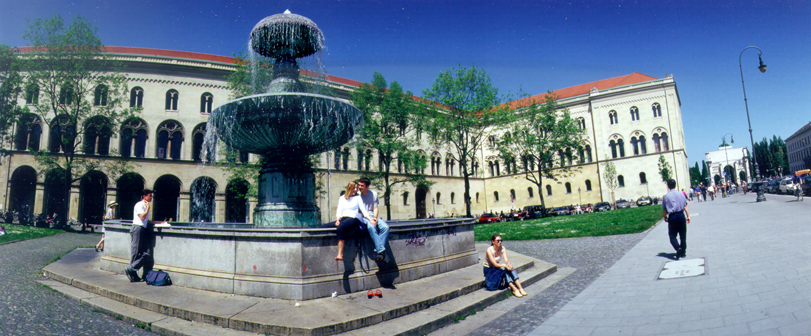
\includegraphics[width=0.31\textwidth]{./gfx/lmu}
\caption{Hovedbyggningen til Ludwig-Maximilians-Universität}
\end{figure}

\section{Utdanningsinsutisjoner}
Det er et stort utvalg av høyskoler i München. De tre største er Ludwig-Maximilians-Universität (LMU), Technische Universität (TUM) og Hochschule München (FHM). LMU og TU er to av Tysklands ni eliteuniversiteter med henholdsvis 45.000 og 25.000 studenter.


LMU - \url{http://www.uni-muenchen.de}\\
TUM - \url{http://portal.mytum.de}\\
FHM - \url{http://www.fh-muenchen.de}\\

Andre:
\begin{enumerate}
\item Hochschule für Politik \\
\url{http://www.hfp.mhn.de}
\item Akademie der Bildenden Künste \\
\url{http://www.adbk.de}
\item Hochschule für Musik und Theater \\
\url{http://website.musikhochschule-muenchen.de/}
\item Bayerische Theaterakademie August Everding \\
\url{http://www.theaterakademie.de}
\item Hochschule für Fernsehen und Film \\
\url{http://www.hff-muenchen.de}
\item Universität der Bundeswehr \\
\url{http://www.unibw.de}
\item Munich Business School \\
\url{http://www.munich-business-school.de}
\end{enumerate}




Informasjon om andre utdanningsinstitusjoner finner man blant annet her:

\url{http://de.wikipedia.org/wiki/M\%C3\%BCnchen#Hochschulen_und_Forschungseinrichtungen/}\\

\url{http://www.muenchen.de/themen/bildung/hochschulen.html}



\subsection{Studietilbud}
Hver høyskole har sitt eget utdanningstilbud som er tilgjengelig på deres respektive internettsider. Her finner man så å si alt en kan tenke seg. 
I 2006 startet begynte høyskolene i München å gå over ifra det gamle Diplom- studiet til Bachelor og Master som vi kjenner i fra Norge.
NB! Enkelte fag kan bare starte til vintersemesteret (bl.a. medisin).



LMU\\
 \url{http://www.uni-muenchen.de/studium/studienangebot/}\\

TUM\\
 \url{http://portal.mytum.de/studium/studiengaenge/index/}\\

FHM \\
\url{http://www.hm.edu/studieninteressiert/studienangebote_1/bersicht_10/}




\section{Søknadsprosessen (ved LMU)}
Det er fire inndelinger for studier ved LMU (for de andre høyskolene i München; sjekk deres internettsider)

1 - Frie studier: søknad til høyskolen (papirformat, karakterer teller ikke)
Her er informasjon og søknadsskjema (link til en annen side): \\
\url{http://www.uni-muenchen.de/studium/studium_int/studium_lmu/bewerbung/}

Søknaden sendes til det Internasjonale Kontoret ved LMU.

Liste over frie studier: \\
\url{http://www.uni-muenchen.de/studium/beratung/vor/studienplatz/studienplatz/zulassungsfrei/}





2 - Lokalt opptaksbegrensede studier må man må søke til høyskolen (karakterer teller)

Man søker kun online, altså ikke papirformat. Her søker man:\\
\url{http://www.uni-muenchen.de/studium/hochschulzugang/bewerb_einschreib/verfahren/online_bewerb/}


3 - Sentralt opptaksbegrensede studier må man er søker til et landsdekkende sentralt opptak, ikke til den lokale høyskolen (lignende samordna opptak - karakterer teller)

Her søker man: \url{http://www.hochschulstart.de}

Informasjon fra LMU om begrensede studier: \\
\url{http://www.uni-muenchen.de/studium/hochschulzugang/bewerb_einschreib/zulassungsbeschr/bundesweit/eu/}

Liste over studier som er begrenset:
\url{http://www.uni-muenchen.de/studium/beratung/vor/studienplatz/studienplatz/zulassungsbeschr/index.html}


4 - For studier med spesielle opptaksprøver ("Studiengang mit Eignungsprüfung"), se studiegang for mer informasjon.



\section{Frister}
Sommersemester:  15. juli
Vintersemester: 15. januar

\begin{figure}[h]
\center

\includegraphics[width=0.31\textwidth]{./gfx/neu}
\caption{Scloß Neuschwanstein ligger ikke langt i fra München}
\end{figure}


\section{Immatrikulasjon (ved LMU)}
De som har søkt og fått plass, trenger bare møte opp til gitt termin med de nødvendige papirene for å skrive seg inn. 
Det er en del papirer en skal ha med seg. Ikke minst diplom på bestått språkprøve. Alt dette foregår i hovedbygningen til LMU.

Nødvendige papirer:
\begin{itemize}
\item Opptaksbrev
\item Online-formular (se nede)
\item Pass
\item Vitnemål (generell studiekompetanse, oversatt til tysk med rett kopi)
\item Sykeforsikringsbevis (se nede, ta med Europeisk helsetrygdkort)
\end{itemize}



Sykeforsikringsbevis får man ved å ta med seg EU Helsekortet sitt til en "krankenkasse" (fritt hvilken) hvor en får et papir som sier "Denne personen er forsikret". De er normalt i samme lokalet og vil være tilgjengelig til samme tid man kan skrive seg inn. Dette er en ren formalitet, koster ingenting og man må ikke nødvendigvis bruke den "Krankenkassen" hvis noe skulle skje. 
Europeisk helsetrygdkort får man fra NAV, men det kan ta opptil to uker fra man søker til man får det i posten. Kortet er gyldig i flere år.

En oversikt over de vanligste Krankenkassene:\\
\url{http://www.uni-muenchen.de/studium/studium_int/studium_lmu/bewerbung/40_eu_auslaender/}

Informasjon om immatrikulasjonen (nødvendige papirer etc.) finner du her:\\
\url{http://www.uni-muenchen.de/studium/studium_int/studium_lmu/immatrikulation/}


Nødvendige dokumenter:\\
\url{http://www.uni-muenchen.de/studium/studium_int/studium_lmu/immatrikulation/grundl_unterlagen/}

Før en går for å immatrikulere seg, må alle ha fylt ut dette online:\\
\url{http://www.uni-muenchen.de/studium/hochschulzugang/bewerb_einschreib/verfahren/online_einschreib/online_einschreibung/}

Som utlendning møter man først opp ved det internasjonale kontoret, for å få vitnemål kontrollert. Deretter går man over til "Studentenkanzlei", som er i nabobygget (sammen med Tyskerne). Informasjon om hvor og når får man i opptaksbrevet.

Avdeling for internasjonale studenter:\\
\url{http://www.uni-muenchen.de/studium/kontakt/international/}

Dette er som sagt hvordan det gjøres ved LMU. Informasjon om hvordan søknadsprosessen og immatrikulasjonen ved andre høyskoler i München foregår finnes på deres respektive internettsider.


\section{Medisinstudiet}

Det er opptak kun en gang i året, om sommeren. Det er omtrent 1000 studenter som begynner på medisin hvert år. Studiet deles inn i en førklinisk del , og en klinisk del. I den førkliniske delen av studiet, som er normert til 2 år, er de tre store og viktige grunnleggende fagene anatomi, fysiologi og biokjemi. Som regel er ikke forelesningene obligatoriske, men i de fleste fagene er det kurs, som en må stille opp på. Prøver er det også, som regel multiple choice.
I feriene må det til sammen utføres 3 måneder med pleietjeneste på et sykehus. I hvilket land denne praksisen avlegges, er det samme, så lenge det er på et sykehus. Når alle prøvene i fagene er bestått, og praksisen gjennomført, kan man melde seg opp til "1. Staatsexamen" også kalt "Physikum". Den består av en skriftlig del (multiple choice) som går over to dager. I tillegg er det en muntlig del. En blir da eksaminert i de tre store fagene.
Når "Physikum" er bestått, dvs. både den skriftlige og muntlige delen, kommer man til den kliniske delen av studiet. Denne er normert til 4 år. Både LMU og TU tilbyr denne delen av studiet. TU er litt mindre. Den kliniske delen er mye mer praktisk rettet. Ikke minst etter innføringen av den nye approbationsordningen, har studentene mye kontakt med pasienter og blir kjent med sykehuset fra innsiden. I feriene må en i løpet av de tre første årene ha 3 måneders praksis på et sykehus og en måneds praksis hos en fastlege. Det siste året av studiet, er et "Praktisches Jahr". Da jobber man på et sykehus, en tredjedel av tiden må en jobbe i kirurgien, en tredjedel i indre medisin, og den siste tredjedelen kan man velge selv hva man vil jobbe med innenfor medisin. Etter det praktiske året, kommer "2. Staatsexamen" også kalt "Hammer Examen". 

Når en har bestått dette, er man ferdig utdannet lege i Tyskland. Vil en tilbake til Norge rett etter studiet, må en ha vanlig norsk turnustjeneste!

Dersom du er interessert i å studere i München eller du allerede har fått studieplass her, må du ikke nøle med å ta kontakt hvis det er noe du lurer på!


\section{Oversetting og kopiering}

Når du skal søke på skoler i utlandet, vil du som oftest bli bedt om å sende med godkjent kopi av vitnemål oversatt til landets språk. Det er mulig at det behandlende organ ved universitetet også aksepterer vitnemål på engelsk. Du vil finne informajson om dette på søknadssidene til universitetet.

Oversettelsen må i de fleste tilfeller være utført av godkjente oversettere.  Oversetting hos byrå eller translatør kan koste fra kr. 600 til kr. 1000 per ark. Spør derfor først ved din videregående skole om de kan oversette vitnemålet ditt til det språket du ønsker det på. Universiteter og høgskoler kan stort sett gi deg en karakterutskrift på andre språk enn norsk. Enkelte vidregående skoler kan oversette vitnemålet til tysk, spør skolen og hør om de kan gjøre det for deg.
Du kan henvende deg direkte til en statsautorisert translatør for å få oversatt vitnemålet ditt, eller du kan bruke et oversetterbyrå som har statsautoriserte translatører. Prisnivået hos byråer vil ligge noe over prisen du får direkte hos en statsautorisert translatør. 


\subsection{Attester}
Hør først med de som har utstedt attesten om de kan skrive den på et annet språk. På lik linje med vitnemål, kan attester også oversettes av en statsautorisert translatør, evt. hos et byrå som har statsautorisert translatør.

\subsection{Rett kopi}
Det er få offentlige kontorer i Norge som idag er villige til å stemple rett kopi. Det er derfor lurt å høre med skolen du har gått på i Norge om de kan ta kopi av vitnemålet og stemple dette for deg. En kan også få rett kopi hos NAV, politiet, flere biblioteker og enkelte kommunesentere.



